\documentclass[xcolor={dvipsnames,table}]{beamer}
\usepackage{epsfig,graphicx}
\usepackage{palatino}
\usepackage{fancybox}
\usepackage{relsize}
\usepackage[procnames]{listings}
\usepackage{hyperref}
\usepackage{qtree} % needed?
\usepackage{booktabs}
\usepackage{dirtree}
\usepackage[normalem]{ulem}
\usepackage{tikz}
\usetikzlibrary{arrows.meta,positioning,calc,fit,shapes.geometric,decorations.pathreplacing}


% fatter TT font
\renewcommand*\ttdefault{txtt}
% another TT, suggested by Alex
% \usepackage{inconsolata}
% \usepackage[T1]{fontenc} % needed as well?


\newcommand{\scale}{0.7}

\newcommand{\todo}[1]{{\emph{TODO: #1}}}
\newcommand{\martin}[1]{{\color{blue} Martin: #1}}
\newcommand{\abcdef}[1]{{\color{red} Author2: #1}}

% uncomment following for final submission
%\renewcommand{\todo}[1]{}
%\renewcommand{\martin}[1]{}
%\renewcommand{\author2}[1]{}

\newcommand{\code}[1]{{\texttt{#1}}}

\hypersetup{
  linkcolor  = black,
%  citecolor  = blue,
  urlcolor   = blue,
  colorlinks = true,
}

\beamertemplatenavigationsymbolsempty
\setbeamertemplate{footline}[frame number]





\newif\ifbook
% shared in slides and book

\lstdefinelanguage{chisel}{
  morekeywords={abstract,case,catch,class,def,%
    do,else,extends,false,final,finally,%
    for,if,implicit,import,match,mixin,%
    new,null,object,override,package,%
    private,protected,requires,return,sealed,%
    super,this,throw,trait,true,try,%
    type,val,var,while,with,yield},
  otherkeywords={=>,<-,<\%,<:,>:,\#,@},
  sensitive=true,
  morecomment=[l]{//},
  morecomment=[n]{/*}{*/},
  morestring=[b]",
  morestring=[b]',
  morestring=[b]"""
}

\usepackage{color}
\definecolor{dkgreen}{rgb}{0,0.6,0}
\definecolor{gray}{rgb}{0.5,0.5,0.5}
\definecolor{mauve}{rgb}{0.58,0,0.82}

% Default settings for code listings
\lstset{%frame=lines,
  language=chisel,
  aboveskip=3mm,
  belowskip=3mm,
  showstringspaces=false,
  columns=fixed, % basewidth=\mybasewidth,
  basicstyle={\small\ttfamily},
  numbers=none,
  numberstyle=\footnotesize\color{gray},
  % identifierstyle=\color{red},
  keywordstyle=\color{blue},
  commentstyle=\color{dkgreen},
  stringstyle=\color{mauve},
  breaklines=true,
  breakatwhitespace=true,
  procnamekeys={def, val, var, class, trait, object, extends},
  procnamestyle=\ttfamily\color{red},
  tabsize=2,
  float
}

\lstnewenvironment{chisel}[1][]
{\lstset{language=chisel,#1}}
{}

\newcommand{\shortlist}[1]{{\lstinputlisting[nolol]{#1}}}

\newcommand{\longlist}[3]{{\lstinputlisting[float, caption={#2}, label={#3}, frame=tb, captionpos=b]{#1}}}


% TikZ for diagrams
\usepackage{tikz}
\usetikzlibrary{positioning, arrows.meta}

% Optional visual tweaks
\tikzset{
    >=Stealth,
    every node/.style={rounded corners=2pt}
}

\title{Agile Hardware Design: Does It Work, and What Did We Build?}
\author{Martin Schoeberl}
\date{\today}
\institute{Technical University of Denmark\\
Embedded Systems Engineering}

\begin{document}

\begin{frame}
\titlepage
\end{frame}




\begin{frame}[fragile]{Outline}
\begin{itemize}
\item Chisel Formal in Chisel 6 and earlier
\item Reflections on agile hardware design
\item Memories
\item Last lecture
\item Today: standup report on your project
\item Week 12: project work
\item Week 13: Final project presentation and demonstration
\begin{itemize}
\item Aim for around 15 minutes
\item Include a demo (on an FPGA)
\item The README is the project report
\item Have it ready the day before the presentation
\item Have a section on AI/LLM usage
\item I am looking at the main branch only!
\end{itemize}
\end{itemize}
\end{frame}

\begin{frame}[fragile]{The New New Product Development Game}
\begin{itemize}
\item by Hirotaka Takeuchi and Ikujiro Nonaka
\item Paper that started the Scrum movement (mid 80s)
\begin{itemize}
\item Move like a rugby team together to reach the aim
\item Instead of a relay race, where runners wait for arrival
\end{itemize}
\item In production, not in software development
\item Observing mostly Japanese, some USA companies
\item Examined multinational companies
\begin{itemize}
\item Fuji-Xerox, Canon, Honda, NEC, Epson, Brother, 3M, Xerox, and Hewlett-Packard
\end{itemize}
\item Available at \href{https://hbr.org/1986/01/the-new-new-product-development-game}{Harward Business Review}
\item Easy reading, give it a try
\end{itemize}
\end{frame}

\begin{frame}[fragile]{New product development processes}
\begin{enumerate}
\item Built-in instability
\item Self-organizing project teams
\item Overlapping development phases
\item ``Multilearning''
\item Subtle control
\item Organizational transfer of learning
\end{enumerate}
\end{frame}

\begin{frame}[fragile]{When is Simulation and Testing Enough?}
\begin{itemize}
\item How much do you need to test?
\item How confident are you?
\begin{itemize}
\item Did you test the corner cases?
\item An issue when the same person did design and tests
\end{itemize}
\item We cannot cover all input possibilities
\item Except in trivial cases
\begin{itemize}
\item Parameters might help
\item Cover all cases for a 4-bit ALU
\item Assume the design also works for 32 bits 
\end{itemize}
\item Any other option?
\end{itemize}
\end{frame}

\begin{frame}[fragile]{Assertions in Chisel}
\begin{itemize}
\item An Assertion statement states assumptions about a program
\item You have seen \code{assert} in Scala in the first lab
\item Can also be used in Chisel
\item Assertion is checked during simulation time
\item Syntax:
\begin{chisel}
  io.sum := io.a + io.b
  assert(io.sum === io.a + io.b, "error message")
\end{chisel}
\end{itemize}
\end{frame}

\begin{frame}[fragile]{Assert Example}
\shortlist{../code/assert.txt}
\end{frame}

\begin{frame}[fragile]{\code{require} vs \code{assert}}
\begin{itemize}
\item Chisel \code{assert} checks value in simulation
\begin{itemize}
\item Emits non-synthesizable Verilog
\item Using a Chisel expression that results in a \code{Bool}
\item Can also have a failure message
\end{itemize}
\item Scala \code{assert} checks value at circuit construction
\item Using a Scala expression that results in a \code{Boolean}
\item Better use Scala's \code{require}
\item \code{require} is used for input sanity checking
\shortlist{../code/fifo_abstract.txt}
\end{itemize}
\end{frame}


\begin{frame}[fragile]{Formal Verification}
\begin{itemize}
\item Simulation explores (only) some test cases
\item Formal verification explores \emph{all} possible behaviors
\item Uses SAT/SMT solvers to prove properties
\begin{itemize}
\item As bounded model checking (BMC)
\end{itemize}
\item Finds corner cases that simulation might miss
\item Sounds a bit too good to be true, right?
\begin{itemize}
\item Might take a long time, days or more
\end{itemize}
\end{itemize}
\end{frame}



\begin{frame}[fragile]{Chisel Formal}
\begin{itemize}
\item Extension of \code{ChiselTest} by Kevin Laeufer
\begin{itemize}
\item Part of his \href{https://www2.eecs.berkeley.edu/Pubs/TechRpts/2024/EECS-2024-157.pdf}{PhD} at UC Berkeley
\end{itemize}
\item Chisel \code{assert} is \emph{formally} checked
\begin{itemize}
\item Up to a bound
\end{itemize}
\item If the proof fails, Chisel formal provides a counter example (as VCD waveform)
\item Install the open \href{https://github.com/Z3Prover/z3}{Z3} theorem prover
\begin{itemize}
\item With your favorite packet manager, e.g., brew, apt,...
\end{itemize}
\end{itemize}
\end{frame}

\begin{frame}[fragile]{Chisel Formal}
\begin{itemize}
\item Import the library
\shortlist{../code/formal_import.txt}
\item Formal is part of ChiselTest (add trait \code{Formal})
\shortlist{../code/formal_class.txt}
\item Use \code{verify} instead of \code{test}
\shortlist{../code/formal_assert.txt}
\item Have the asserts in your module
\end{itemize}
\end{frame}

\begin{frame}[fragile]{Access the History}
\begin{itemize}
\item \code{past()} allows us to make assamptions over time
\item If \code{in} was 10 last cycle, then \code{out} must be 11 now
\shortlist{../code/formal_past.txt}
\item A signal must stay stable, be the same as in the last cycle
\shortlist{../code/formal_stability.txt}
\item With \code{past(x)} call we get the value of \code{x} from the last clock cycle
\end{itemize}
\end{frame}

\begin{frame}[fragile]{Past Example}
\shortlist{../code/formal_past_example.txt}
\end{frame}

\begin{frame}[fragile]{Assumptions}
\begin{itemize}
\item We can limit the search space
\item Assuming that some (input) signals have restricted values
\item Assume that a signal will never be zero:
\shortlist{../code/formal_assume.txt}
\end{itemize}
\end{frame}

\begin{frame}[fragile]{Assume Example}
\shortlist{../code/formal_assume_example.txt}
\end{frame}

\begin{frame}[fragile]{More Functions}
\begin{itemize}
\item Synthactic sugar for \code{past}
\item changed
\item fell
\item rose
\item stable
\item See \href{https://www.javadoc.io/doc/edu.berkeley.cs/chiseltest_2.12/latest/chiseltest/formal/index.html}{Javadoc}
\end{itemize}
\end{frame}

\begin{frame}[fragile]{Limits to Bounded Model Checking}
\begin{itemize}
\item BMC will check your design only for the first N cycles
\item Can fail in clock cycle N+1
\item Only checks your assertions
\item They need to be correct
\end{itemize}
\end{frame}

\begin{frame}[fragile]{Other Options}
\begin{itemize}
\item Synopsys and Cadence have for sure formal verifiers
\item \href{https://github.com/YosysHQ/sby}{Sby} is a free, open-source verification tool
\item Part of YosysHQ
\item See Matt Venn \href{https://www.youtube.com/watch?v=B1KX2rFJqVE}{explaining it}
\item \href{https://symbiyosys.readthedocs.io/en/latest/index.html}{SymbiYosys (sby) Documentation}
\end{itemize}
\end{frame}

%\begin{frame}[fragile]{Next Week}
%\begin{itemize}
%\item Guest lecture by Frans Skarman
%\item On Spade, a new HDL
%\item Frans developed also Surfer, the new waveform viewer
%\begin{itemize}
%\item Check out the VSC plugin (show it)
%\end{itemize}
%\item Please \href{https://docs.spade-lang.org/agile/quick_setup.html}{setup Spade}
%\end{itemize}
%\end{frame}

\begin{frame}[fragile]{The Final Sprints}
\begin{itemize}
\item Make the design correct
\item Check the hardware it generates (FPGA reports)
\item Make the results reproducible (README instructions)
\begin{itemize}
\item Can someone else understand your project?
\item Can someone else simulate your project?
\end{itemize}
\item What is the biggest remaining uncertainty in your project?
\end{itemize}
\end{frame}

\begin{frame}[fragile]{XXX}
\begin{itemize}
\item xxx
\item xxx
\item xxx
\begin{itemize}
\item xxx
\end{itemize}
\item xxx
\item xxx
\end{itemize}
\end{frame}

\begin{frame}[fragile]{XXX}
\begin{itemize}
\item xxx
\item xxx
\item xxx
\begin{itemize}
\item xxx
\end{itemize}
\item xxx
\item xxx
\end{itemize}
\end{frame}

\begin{frame}[fragile]{XXX}
\begin{itemize}
\item xxx
\item xxx
\item xxx
\begin{itemize}
\item xxx
\end{itemize}
\item xxx
\item xxx
\end{itemize}
\end{frame}

\begin{frame}[fragile]{Memory}
\begin{itemize}
\item Sometimes we need to store values/state
\item State machine, register file, instruction and data memories,...
\item Three or more options
\begin{itemize}
\item Flip-flops
\item (Latches)
\item SRAM blocks
\item External memory
\end{itemize}
\item Which to use when?
\end{itemize}
\end{frame}

\begin{frame}[fragile]{Memory in Chisel}
\begin{itemize}
\item Chisel has three constructs for storage elements
\begin{itemize}
\item \code{Reg(Vec(...))}
\item \code{Mem}
\item \code{SyncReadMem}
\end{itemize}
\item What is the difference?
\item What maps to what?
\item What is the read latency?
\end{itemize}
\end{frame}

\begin{frame}[fragile]{Memory}
\begin{itemize}
\item Registers are storage elements == memory
\item Just use a \code{Reg} of a \code{Vec}
\item This is 1 KiB of memory
\begin{chisel}
  val memoryReg = Reg(Vec(1024, UInt(8.W)))
  // writing into memory
  memoryReg(wrAddr) := wrData
  // reading from the memory
  val rdData = memoryReg(rdAddr)
\end{chisel}
\item Simple, right?
\item But is this a good solution?
\end{itemize}
\end{frame}

\begin{frame}[fragile]{A Flip-Flop}
\begin{itemize}
\item Remember the circuit of a register (flip-flop)?
\item Two latches: \href{https://en.wikipedia.org/wiki/Flip-flop_(electronics)#Master%E2%80%93slave_edge-triggered_D_flip-flop}{master and slave}
\item One (enable) latch can be built with 4 NAND gates
\item A NAND gate needs 4 transistors; an inverter needs 2 transistors
\item A flip-flop needs 36 transistors (for a single bit)
\item Can we do better?
\end{itemize}
\end{frame}

\begin{frame}[fragile]{A Memory Cell}
\begin{itemize}
\item A single bit can be stored in \href{https://en.wikipedia.org/wiki/Static_random-access_memory#/media/File:SRAM_Cell_(6_Transistors).svg}{6 transistors}
\begin{itemize}
\item Corsscoupled invertes plus access transistors
\end{itemize}
\item That is how larger memories are built
\item FPGAs have this type of on-chip memories
\item Usually many of them in units of 2 KiB or 4 KiB
\item We need some Chisel code to represent it
\item More memory needs an external chip
\item Then we need to interface this memory with the FPGA
\end{itemize}
\end{frame}

\begin{frame}[fragile]{SRAM Memory}
\begin{itemize}
\item RAM stands for random access memory
\item SRAM stands for static RAM
\item There is also something called DRAM for dynamic RAM
\begin{itemize}
\item Uses a capacitor and a transistor
\item DRAM is smaller than SRAM
\item But needs refreshes
\item Different technology than technology for logic
\end{itemize}
\item All on-chip memory is SRAM (today)
\end{itemize}
\end{frame}

\begin{frame}[fragile]{Memory Interface}
\begin{itemize}
\item Interface
\begin{itemize}
\item Address input (e.g., 10 bits for 1 KiB)
\item Write signal (e.g., we)
\item Data input
\item Data output
\end{itemize}
\item May share pins for the data input and output (tri-state)
\item May have read and write addresses
\begin{itemize}
\item A so-called dual ported memory
\item Can do a read and a write in the same clock cycle
\end{itemize}
\end{itemize}
\end{frame}


\begin{frame}[fragile]{On-Chip Memory}
\begin{itemize}
\item SRAM by itself is asynchronous
\item No clock, just the correct timing
\item Apply the address and after some time the data is valid
\item But one can add input registers, which makes it a synchronous SRAM
\item Current FPGAs have synchronous memories only
\item This means the result of a read is available one clock cycle after the address is given
\begin{itemize}
\item This is different from the use of flip-flops (\code{Reg(Vec(..))})
\end{itemize}
\item FPGAs usually have dual-ported memories
\end{itemize}
\end{frame}

\begin{frame}[fragile]{Synchronous Memory}
\begin{figure}
  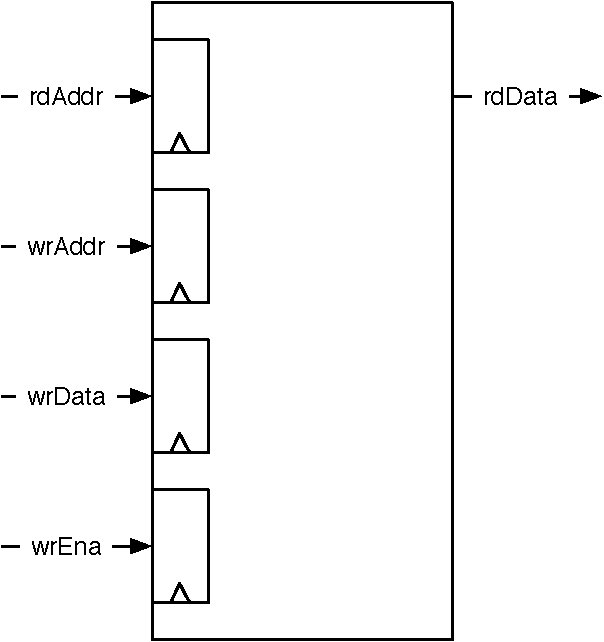
\includegraphics[scale=\scale]{../figures/memory}
\end{figure}
\end{frame}

\begin{frame}[fragile]{Use of a Chisel SyncReadMem}
\shortlist{../code/memory.txt}
\end{frame}

\begin{frame}[fragile]{Read-During-Write}
\begin{itemize}
\item What happens when one writes to and reads from the same address?
\item Which value is returned?
\item Three possibilities:
\begin{enumerate}
\item The newly written value
\item The old value
\item Undefined (mix of old and new)
\end{enumerate}
\item Depends on technology, FPGA family, ...
\item We want to have a defined read-during-write
\item We add hardware to \emph{forward} the written value
\end{itemize}
\end{frame}

\begin{frame}[fragile]{Condition for Forwarding}
\begin{itemize}
\item If read and write addresses are equal
\item If write enable is true
\item Multiplex the output to take the new write value instead of the (old) read value
\item Delay that forwarded write value to have the same timing
\end{itemize}
\end{frame}

\begin{frame}[fragile]{Memory with Forwarding}
\begin{figure}
  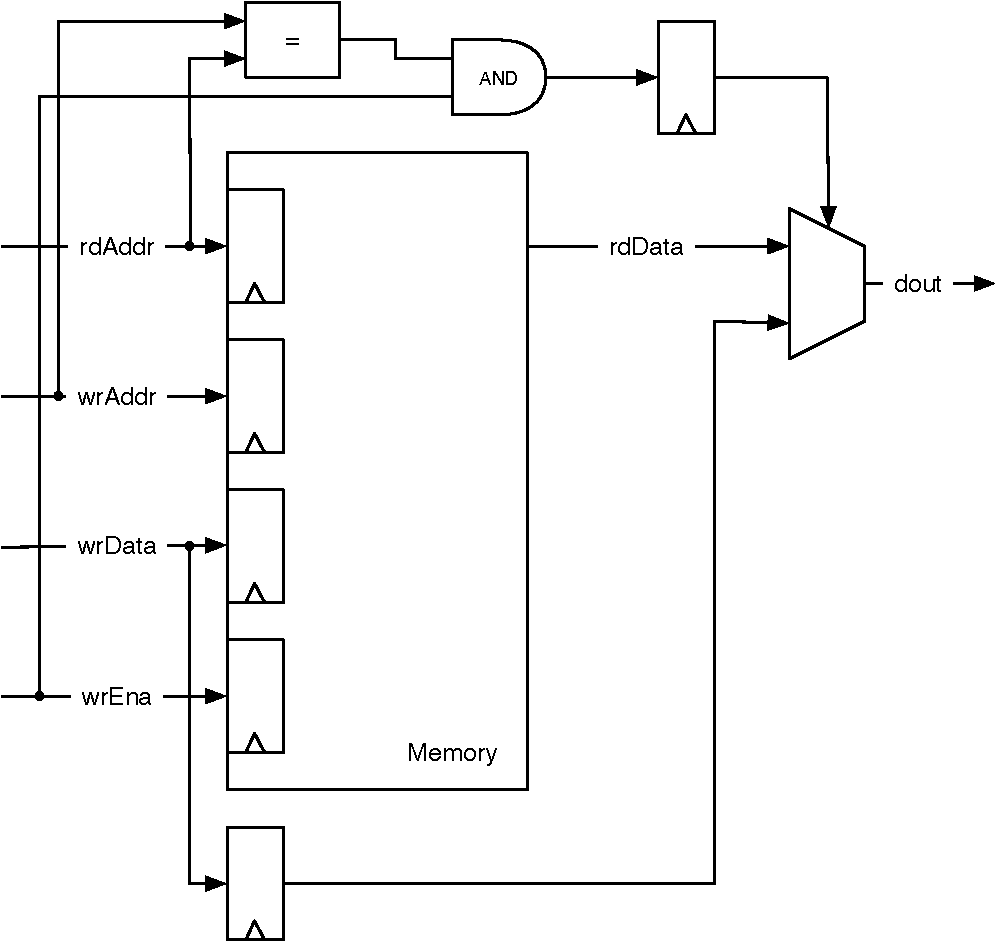
\includegraphics[scale=0.5]{../figures/memory-forwarding}
\end{figure}
\end{frame}

\begin{frame}[fragile]{Forwarding in Chisel}
\begin{chisel}
  val mem = SyncReadMem(1024, UInt(8.W))

  val wrDataReg = RegNext(io.wrData)
  val doForwardReg = RegNext(io.wrAddr === io.rdAddr && io.wrEna)

  val memData = mem.read(io.rdAddr)

  when(io.wrEna) {
    mem.write(io.wrAddr, io.wrData)
  }

  io.rdData := Mux(doForwardReg, wrDataReg, memData)
\end{chisel}
\end{frame}


\begin{frame}[fragile]{External Memory}
\begin{itemize}
\item On-chip memory is limited
\item We can add an external memory chip
\begin{itemize}
\item Is cheaper than FPGA on-chip memory
\end{itemize}
\item Sadly, the Basys 3 board has no external memory
\item The simplest memory is an asynchronous SRAM
\item You can add an external memory via SPI on the connectors
\end{itemize}
\end{frame}


\begin{frame}[fragile]{Documentation}
\begin{itemize}
\item Summarize the purpose of your project
\item Instruct how to use it
\item List dependencies
\item Good documentation:
\begin{itemize}
\item May attract users
\item May even attract contributors
\item Forces you to rethink your project
\end{itemize}
\item Start early with the documentation (latest today!)
\end{itemize}
\end{frame}

\begin{frame}[fragile]{README.md Documentation}
\begin{itemize}
\item Well-suited for small to medium projects
\item Immediately visible on GitHub
\item Use Markdown for simple formatting
\item Include figures, best in SVG
\item README is the report and part of the grade
\item Up to now, not much is going on (mostly)
\begin{itemize}
\item Do not wait till the final week!
\item We need to read it on Monday before the final presentation
\item Commit the latest changes on Sunday 29/11 night
\end{itemize}
\item BTW, do you have GitHub Actions set up for CI?
\end{itemize}
\end{frame}

\begin{frame}[fragile]{Summary}
\begin{itemize}
\item We had the theory on formal last week
\item Today, simple examples with Chisel 6 and Z3
\item Formal verification is the next step in testing
\item It is another tool in your toolbox
\item Easy to include in your continuous integration on GitHub
\item There is a lab for Formal in Chisel 6 \href{https://github.com/schoeberl/agile-hw/tree/main/lab8}{lab} exercises for you
\end{itemize}
\end{frame}


\end{document}

\begin{frame}[fragile]{XXX}
\begin{itemize}
\item xxx
\item xxx
\item xxx
\begin{itemize}
\item xxx
\end{itemize}
\item xxx
\item xxx
\end{itemize}
\end{frame}

\begin{frame}[fragile]{Title}
\begin{itemize}
\item abc
\end{itemize}
\end{frame}
